\section{Allgemeine Zufallsvariablen}

\subsection{Grundbegriffe}
\begin{definition}[\textbf{Zufallsvariable}]
Sein $(\Omega,\mathcal{F}, P)$ ein Wahrscheinlichkeitsraum. Eine \textit{Zufallsvariable} (ZV) auf $\Omega$ ist eine messbare Funktion $X:\Omega \to \R$, das bedeutet, dass die Menge $\{X \leq t\} = \{ \omega \with X(\omega) \leq t\}$ für jedes $t$ ein beobachtbares Ereignis, also $\in \mathcal{F}$ sein muss. \\
Die \textit{Verteilungsfunktion} (VF) von $X$ ist die Abbildung $F_X:\R\to [0,1]$ mit
$$ t \mapsto F_X(t) := P[X \leq t] := P[\{ \omega \with X(\omega) \leq t\}]$$
\end{definition}
Wir betrachten nur messbare Zufallsvariablen in dieser Vorlesung.

\begin{satz}[\textbf{Eigenschaften der Verteilungsfunktion}]
$F_X$ hat folgende Eigenschaften:
\begin{itemize}
\item[(i)] $F_X$ ist \textit{wachsend} und \textit{rechtsstetig}: $F_X(s) \leq F_X(t)$ für $s\leq t$ und $F_X(u) \to F_X(t)$ für $u\to t$ mit $u>t$.
\item[(ii)] $lim_{t\to -\infty} F_X(t) = 0$ und $\lim_{t\to\infty} F_X(t) =1 $
\end{itemize}
\end{satz}

Das stochastische Verhalten einer ZV $X$ wird durch die \textit{Verteilung} beschrieben, d.h. das Wahrscheinlichkeitsmass $\mu_X$, welches durch $\mu_X(B) = P[X\in B]$ definiert ist. Sobald die Verteilungsfunktion $F_X$ bekannt ist, ist das Mass $\mu_X$ festgelegt, nämlich durch den Zusammenhang
$$F_X(t) = \mu_X\left((-\infty, t]\right)$$
Anstelle der Gewichtsfunktion aus dem diskreten Fall verwenden wir die \textit{Dichtefunktion}, sofern diese existiert.

\begin{definition}[\textbf{Dichtefunktion}]
Eine ZV $X$ mit Verteilungsfunktion $F_X(t) = P[X \leq t]$ heisst \textit{(absolut) stetig} mit Dichtefunktion $f_X:\R\to [0,\infty)$, falls gilt
$$ F_X(t) = \int \limits_{-\infty}^t f_X(s) \: ds \quad \quad \mbox{ für alle } t \in \R. $$
\end{definition}
\underline{Bemerkung:} $X$ heisst stetig, falls $F_X$ nur stetig ist. Eine ZV $X$ mit einer Dichte hat aber eine VF $F_X$, die fast überall differenzierbar ist. Dafür verwenden wir den Begriff \textit{\textcolor{blue}{stetig mit Dichte}}.

\begin{satz}[\textbf{Eigenschaften der Dichte}]
Die Dichtefunktion $f_X$ hat folgende Eigenschaften:
\begin{itemize}
\item[(i)] $f_X \geq 0$ und $f_X = 0$ ausserhalb des Wertebereichs $\mathcal{W}(X)$
\item[(ii)] $ \int \limits_{-\infty}^{\infty} f_X(s) \: ds = 1$ (dies folgt aus Eigenschaft (ii), 2. GW von der Verteilungsfunktion.)
\end{itemize}
In beinahe allen praktischen Beispielen ist $f_X$ zusätzlich stetig oder zumindest stückweise stetig.
\end{satz}

Die Dichtefunktion ist beinahe analog zur Gewichtsfunktion für diskrete Zufallsvariablen, jedoch unterscheidet sie sich in Punktwahrscheinlichkeiten. Es gilt
\begin{align*}
P[a < X \leq b] &= P[X \leq b] - P[X \leq a] = F_X(b) - F_X(a) = \int \limits_a^b f_X(s) \: ds \\&\implies P[X\in B] = \int\limits_B f_X(s)\: ds
\end{align*}
und betrachtet man nun einen Grenzwert, so erhält man
$$ \lim_{\epsilon \to 0^+} P[t-\epsilon < X \leq t + \epsilon] = \lim_{\epsilon \to 0^+} \int \limits_{t-\epsilon}^{t+\epsilon} f_X(s) \: ds = 0 = P[X=t]$$
Damit ist die Punktwahrscheinlichkeit an jedem Punkt = 0. Jedoch gilt für kleine $\epsilon$ (wir verwenden hier $\epsilon= dt$) das Folgende:
$$ P\left[X\in (t,t+dt]\right] = f_X(t) dt$$
In allen vernünftigen Situationen gilt also der folgende Zusammenhang zwischen Dichtefunktion und Verteilung:
\begin{center}
Dichtefunktion = Ableitung der Verteilungsfunktion
\end{center}
Vom diskreten zum stetigen Fall kommt man , indem Summen durch Integrale und die Gewichtsfunktion durch die Dichte ersetzt.

\subsection{Wichtige stetige Verteilungen}

\subsubsection{Gleichverteilung}
Gleichverteilung auf Intervall $[a,b]$ modelliert die zufällige Wahl eines Punktes in $[a,b]$
\begin{itemize}
\item \textbf{Wertebereich:} $\mathcal{W}(X) = [a,b]$
\item \textbf{Dichtefunktion:} $f_X(t) = \begin{cases} \frac{1}{b-a} & \mbox{für } a \leq t \leq b \\ 0 &  \mbox{sonst} \end{cases}$
\item \textbf{Verteilungsfunktion:} $F_X(t) = \begin{cases} 0 & \mbox{für } t < a \\ \frac{t-a}{b-a} & \mbox{für } a \leq t \leq b \\ 1 & \mbox{für } t > b \end{cases}$
\item \textbf{Notation:} $X \sim \mathcal{U}(a,b)$ wobei das $\mathcal{U}$ für uniform steht.
\end{itemize}
Ein wichtiger Spezialfall ist $\mathcal{U}(0,1)$, wodurch die Formeln auch etwas einfacher aussehen.
\begin{center}
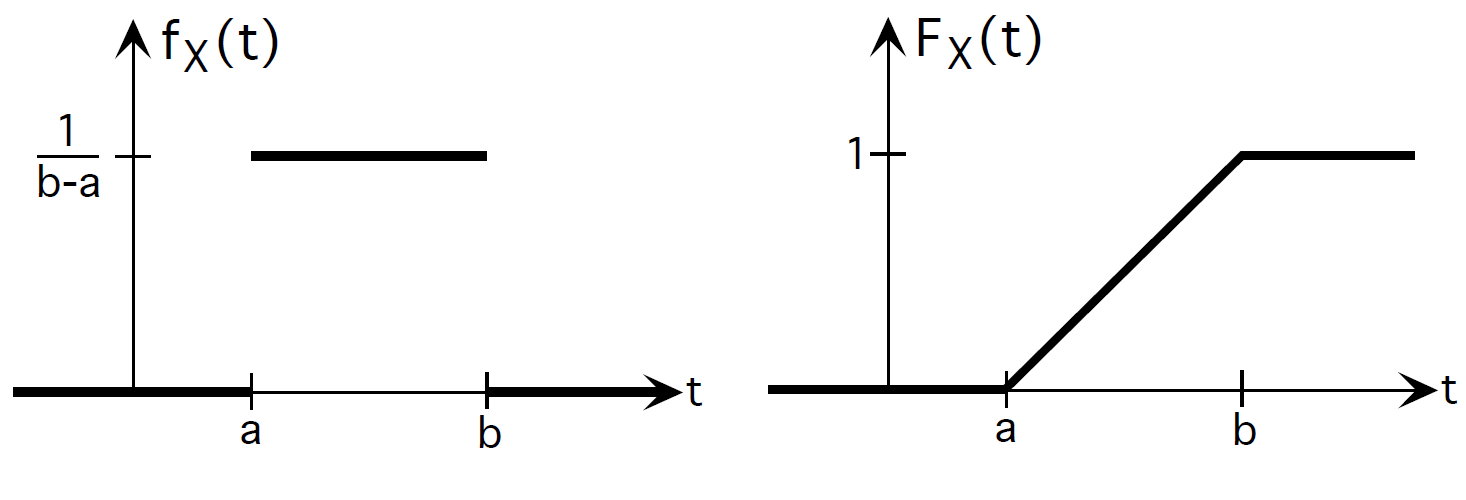
\includegraphics[scale=0.2]{gleichverteilung.png}
\end{center}

\subsubsection{Exponentialverteilung}
Exponentialverteilung mit Parameter $\lambda >0$ ist stetiges Analogon zur geometrischen Vereteilung und ist ebenfalls ein Modell für Wartezeiten oder Lebensdauer
\begin{itemize}
\item \textbf{Wertebereich:} $\mathcal{W}(X) = [0, \infty)$
\item \textbf{Dichtefunktion:} $ f_X(t) = \begin{cases} \lambda e^{-\lambda t} & \mbox{für } t \geq 0 \\ 0 & \mbox{für } t < 0 \end{cases}$
\item \textbf{Verteilungsfunktion:} $F_X(t) = \int\limits_{-\infty}^t f_X(s) \: ds = \begin{cases} 1 - e^{-\lambda t} & \text{ für } t \geq 0 \\ 0 & \text{ für } t < 0 \end{cases}$
\item \textbf{Notation:} $X \sim Exp(\lambda)$
\item die Verteilung ist \textit{gedächtnislos} $\implies$ $P[X > t+ s \with X > s ] = P[X>t]$
\end{itemize}
Analog zur geometrischen Verteilung ein Modell für Wartezeiten oder Lebensdauer.
\begin{center}
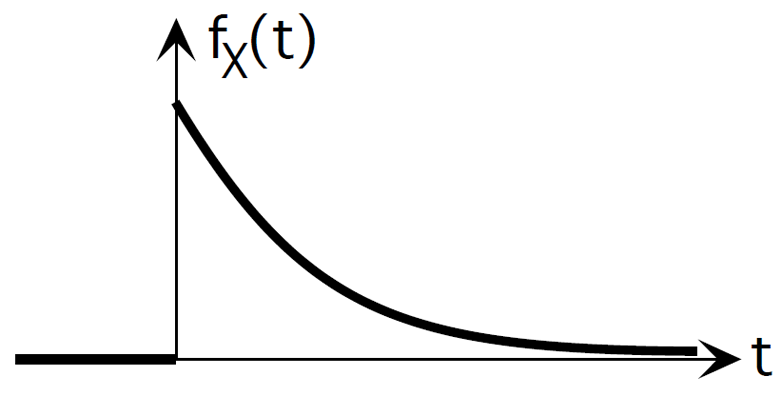
\includegraphics[scale=0.2]{exponentialverteilung.png}
\end{center}

\subsubsection{Gamma-Verteilung}
Die \textit{Gamma-Verteilung} ist eine Verallgemeinerung der Exponentialverteilung mit Parametern $\alpha, \lambda > 0$. Sie wird in der Warteschlangentheorie verwendet.
\begin{itemize}
\item \textbf{Wertebereich:} $\mathcal{W}(X) = \R^+$
\item \textbf{Dichtefunktion:} $f(x) = \frac{1}{\Gamma(\alpha)}\lambda^\alpha x^{\alpha -1} e^{-\lambda x}$ für $z \geq 0$.
\item \textbf{Erwartunsgwert:} $\E[X] = \frac{\alpha}{\lambda}$
\item \textbf{Varianz:} $\mathrm{Var}[X] = \frac{\alpha}{\lambda^2}$
\item \textbf{Notation:} $X \sim Ga(\alpha, \lambda)$
\end{itemize}
wobei die Gamma-Funktion die reelle Erweiterung der Fakultätsfunktion ist:
$$ \Gamma(\alpha) := \int \limits_0^\infty u^{\alpha -1}e^{-u} \ du \quad \quad \mbox{ für } \alpha > 0$$ \underline{Bemerkung:} Die Gamma-Funktion mit Parameter $\alpha =1$ entspricht exakt der Exponentialfunktion. Eine Summe von $n$ unabhängigigen Zufallsvariablen mit Verteilung $Exp(\lambda)$ ist $Ga(n, \lambda)$-verteilt.

\subsubsection{Normalverteilung}
Normalverteilung oder \textit{Gauss-Verteilung} nimmt zwei Parameter $\mu \in \R,\: \sigma^2 > 0$. Ihre Dichte ist symmetrisch um $\mu$ und hat eine glockenförmige Gestalt.
\begin{itemize}
\item \textbf{Wertebereich:} $\mathcal{W}(X) = \R$
\item \textbf{Dichtefunktion:} $f_X(t) = \frac{1}{\sigma \sqrt{2\pi}}e^{- \frac{(t-\mu)^2}{2\sigma^2}}$ für $t\in \R$
\item \textbf{Erwartungswert:} $\E[X] = \mu$ und \textbf{Varianz:} Var$[X] = \sigma^2$
\item \textbf{Verteilungsfunktion:} entspricht dem Integral von der Dichtefunktion über dem Intervall $[-\infty, t)$, es existiert jedoch kein geschlossener Term.
\item \textbf{Notation:} $X \sim \mathcal{N}(\mu, \sigma^2)$
\end{itemize}
\begin{center}
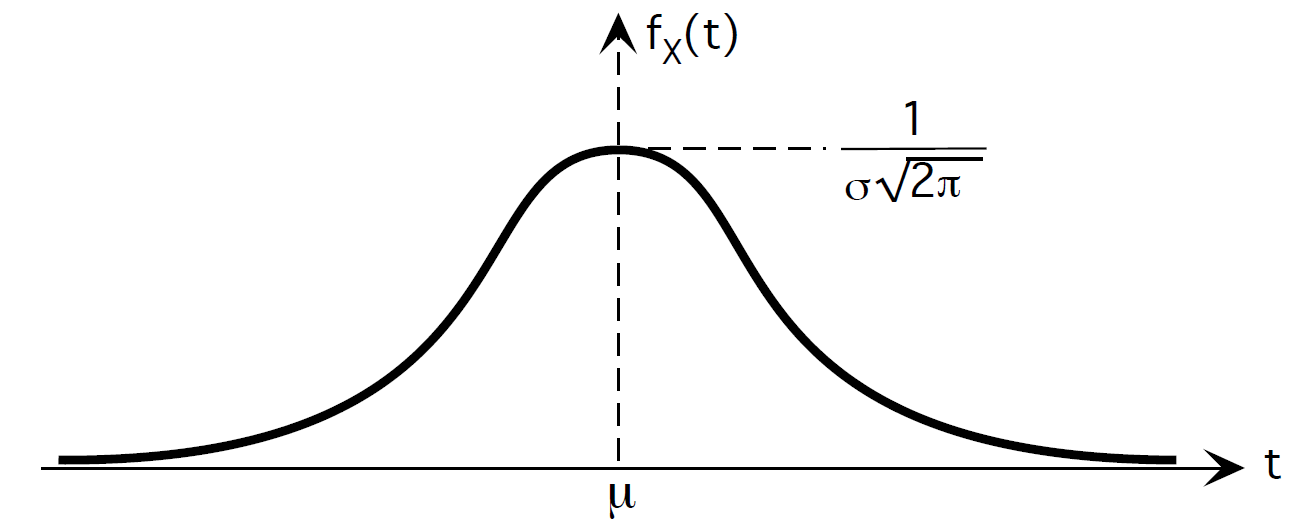
\includegraphics[scale=0.3]{normalverteilung.png}
\end{center}
Mit einer Normalverteilung können z.b: die Streuung von Messwerten um ihren Mittelwert, Gewichte bzw. Grössen in Bevölkerungen, Leistungen in IQ-Tests und viele mehr modelliert werden. Der Grund für die Wichtigkeit der Normalverteilung liegt im \textit{Zentralen Grenzwertsatz}, der in Kapitel 5 besprochen wird.

\subsubsection{Standard-Normalverteilung}
Die \textit{Standard-Normalverteilung} gibt die beiden Parameter vor: $\mu = 0$ und $\sigma^2 = 1$.
\begin{itemize}
\item \textbf{Dichtefunktion:} $\phi(t) = \frac{1}{\sqrt{2\pi}}e^{-\frac{t^2}{2}}$
\item \textbf{Verteilungsfunktion:} Wieder existiert kein geschlossener Ausdruck, jedoch ist das Integral \textit{tabelliert}:
$$ \Phi(t) = \int\limits_{-\infty}^t \phi(s) \: ds = \frac{1}{\sqrt{2\pi}} \int\limits_{-\infty}^t e^{-\frac{s^2}{2}}\: ds$$
\end{itemize}
\underline{Wichtig:} $X \sim \mathcal{N}(\mu, \sigma^2) \implies  \frac{X-\mu}{\sigma} \sim \mathcal{N}(0,1)$. Daraus folgt unmittelbar, dass es ausreicht, nur die Werte von $\Phi(t)$ zu tabellieren, denn es gilt:
$$ F_X(t) = P[X \leq t] = P\left[ \frac{X-\mu}{\sigma} \leq \frac{t-\mu}{\sigma} \right] = \Phi\left(\frac{t-\mu}{\sigma}\right)$$


\subsection{Erwartungswerte}
Eine beliebige reellwertige ZV $X$ kann immer durch eine Folge diskreter ZV approximiert werden. Ist bspw. $X \geq 0$, dann kann man 
$$ X_N := \sum_{k=1}^{n2^n} \frac{k-1}{2^n}I_{\{\frac{k-1}{2^n} \leq X \leq \frac{k}{2^n}\}} + nI_{\{X \geq n\}}$$
für $X_n \nearrow X$ wählen und erhält den Erwartungswert als $$ \E[X] := \lim_{n\to\infty} \E[X_n]$$
Für allgemeine Zufallsvariablen zerlegt man $X = X^+ - X^- := \max{(X,0)} - \max{(-X,0)}$ mit $X^+, X^- \geq 0$ und setzt dann $\E[X] = \E[X^+] - \E[X^-]$. Sind diese beiden Erwartungswerte nicht endlich, so existiert der Erwartungswert von $X$ nicht (in $\R$).\\

\underline{\textbf{Erwartungswert berechnen:}} Ist $X$ stetigt mit einer Dichte $f_X(x)$, so gilt (sofern konvergent):
$$ \E[X] = \int \limits_{-\infty}^{\infty} x \cdot f_X(x) \: dx$$
\underline{\textit{Cauchy-Verteilung:}} $\mathcal{W}(X) = \R$ mit Dichte $f_X(x) = \frac{1}{\pi}\frac{1}{1+x^2}$ und Verteilung $F_X(x) = \frac{1}{2} + \frac{1}{\pi} \arctan(x)$. Es gilt, dass für zwei unabhängige, $\mathcal{N}(0,1)$-verteilte ZV $X,Y$ ihr Quotient $Z := X/Y$ gerade \textit{Cauchy-verteilt} ist. Die Charakteristik liegt darin, dass die Dichte für $|x| \to \infty$ sehr langsam gegen 0 geht, d.h. auch sehr grosse Werte nocht mit substantieller Wahrscheinlichkeit angenommen werden. Ein Erwartungswert existiert nicht.\\

\begin{satz}
Seien $X$ und $Y=g(X)$ zwei ZV. Ist $X$ stetig mit Dichte $f_X(x)$ dann gilt (sofern das Integral konvergiert)
$$ \E[Y] = \E[g(X)] = \int \limits_{-\infty}^{\infty} g(x) \cdot f_X(x) \: dx$$
\end{satz}
Weitere Eigenschaften für Erwartungswerte gelten analog zum diskreten Fall, einzig die konkreten Berechnungen unterscheiden sich.

\subsection{Momente \& Absolute Momente}
\begin{definition}[\textbf{Moment}]
Sei $X$ eine Zufallsvariable und $p\in R_+$. Wir definieren:
\begin{itemize}
\item \textit{das} $p$\textit{-te absolute Moment von} $X$ durch $M_o := \E[|X|^p ]$ (kann $\infty$ sein)
\item falls $M_n < \infty$ für ein $n$, dann ist das $n$\textit{-te Moment von} $X$ durch $m_n:= \E[X^n]$ definiert.
\end{itemize}
\end{definition}
Damit folgt sofort:
\begin{korollar}
$M_n < \infty$ für $n\in\N \implies |m_n| \leq M_n$
\end{korollar}
Hat $X$ eine Dichte $f_X$, dann gilt zudem für das absolute Moment
$$ M_p = \int \limits_{-\infty}^\infty |x|^p f_X(x) \ dx$$ 
Gilt dann $M_n < \infty$ für ein $n\in\N$, dann können wir auch das $n$-te Moment per Integral bestimmen:
$$ m_n = \int \limits_{-\infty}^{\infty} x^n f_X(x) \ dx $$

\begin{satz}
Sei $X$ ZV und $p,q \in R_+$. Dann:
$$ p \leq q \; \land \; M_q < \infty \implies M_p < \infty$$
\end{satz}
\subsection{Gemeinsame Verteilungen, Unabhängige Zufallsvariablen}

\begin{definition}[\textbf{Gemeinsame Verteilung}]
Die \textit{gemeinsame Verteilungsfunktion} von $n$ ZV $X_1,\dots, X_n$ ist die Abbildung $F:\R^n \to [0,1]$ mit:
$$ (x_1,\dots, x_n) \mapsto F(x_1, \dots, x_n) := P[X_1 \leq x_1, \dots, X_n \leq x_n]$$
Lässt sich $F$ für eine Funktion $f:\R^n \to [0, \infty)$ schreiben als 
$$ F(x_1,\dots, x_n) = \int\limits_{-\infty}^{x_1} \dots \int \limits_{-\infty}^{x_n} f(t_1, \dots, t_n) dt_n \dots dt_1 $$
dann heisst $f(x_1,\dots, x_n)$ die \textit{gemeinsame Dichte} von $X_1, \dots, X_n$.
\end{definition}

\begin{korollar}[\textbf{Eigenschaften der Dichte}]
Für die gemeinsame Dichte von $X_1,\dots,X_n$ gilt:
\begin{itemize}
\item[(i)] $f(x_1,\dots, x_n) \geq 0$ und $=0$ ausserhalb $\mathcal{W}(X_1, \dots, X_n)$
\item[(ii)] $ \iiint \limits_{\R^n} f(x_1, \dots, x_n) dx_n \dots dx_1 = 1$
\item[(iii)] $P[(X_1,\dots, X_n) \in A] = \iiint \limits_{(x_1,\dots,x_n) \in A} f(x_1, \dots, x_n) dx_n \dots dx_1$ für $A\subseteq \R^n$.
\end{itemize}
\end{korollar}

\begin{definition}[\textbf{Randverteilung}]
Haben $X,Y$ die gemeinsame Verteilungsfunktion $F$, dann sind $F_X:\R\to[0,1]$ und $F_Y:\R\to[0,1]$ die Verteilungsfunktionen der \textit{Randverteilung} von $X$ bzw. $Y$ und sind definiert als:
$$ x \mapsto F_X(x) := P[X \leq x] = P[X \leq x, Y < \infty] = \lim_{y\to \infty} F(x,y)$$
$$ y \mapsto F_Y(y) := P[Y \leq y] = P[X < \infty, Y \leq y] = \lim_{x\to \infty} F(x,y)$$
Haben $X,Y$ eine gemeinsame Dichte $f$, dann haben auch die Randverteilungen Dichten $f_X:\R\to [0, \infty)$ und $f_Y:\R \to [0, \infty)$ mit
$$ f_X(x) = \int\limits_{-\infty}^{\infty} f(x,y) dy \quad \quad \quad \quad \quad f_Y(y) = \int \limits_{-\infty}^{\infty} f(x,y) dx$$
\end{definition}

\begin{definition}[\textbf{Unabhängigkeit}]
Die ZV $X_1,\dots,X_n$ heissen \textit{unabhängig} $LLRA$ $F(x_1,\dots,x_n) = F_{X_1}(x_1) \cdots F_{X_n}(x_n)$.\\
Hat man stetige Zufallsvariablen mit Dichten, dann ist die gemeinsame Dichtefunktion das Produkt der Randdichten, also
$$ f(x_1, \dots, x_n) = f_{X_1}(x_1) \cdots f_{X_n}(x_n)$$
\end{definition}

\subsection{Bedingte Verteilungen usw}

\begin{definition}[\textbf{Bedingte Dichte und Erwartungswert}]

$$ f_{X_1 \mid X_2}(x_1\mid x_2) = \frac{f_{X_1, X_2}(x_1, x_2)}{f_{X_2}(x_2)}$$
$$ E[X_1 \mid X_2](x_2) = \int x_1 f_{X_1 \mid X_2}(x_1\mid x_2)\ dx_1$$
Mit Trick:
\begin{align*}
	E[X_1] = E[E[X_1 \mid X_2]] &= \int E[X_1 \mid X_2](x_2) f_{X_2}(x_2) dx_2\\
	&=\int \int x_1 f_{X_1, X_2}(x_1, x_2) dx_1 dx_2
\end{align*}
Anm. $E[X_1 \mid X_2](x_2) = E[X_1 \mid X_2=x_2]$ 
\end{definition}

\subsection{Funktionen und Transformationen von Zufallsvariablen}
\subsubsection*{Summen}
Für $Z=X+Y$ suchen wir die Verteilungsfunktion $F_Z(z) = P[Z \leq z] = P[X+Y \leq z]$. Dies kann man als Punktemenge im $\R^2$ auffassen, nämlich $A_z := \{(x,y) \in \R^2 \with x+y \leq z\}$. Damit ist $F_Z(z) = P[(X,Y) \in A_z]$. Damit erhält man 
$$F_Z(z) = \int \limits_{-\infty}^\infty \int \limits_{-\infty}^{z-x} f(x,y) \ dy \ dx $$
Substituiere nun $v=x+y \Rightarrow y = v-x, dy = dv$ so erhält man
\begin{align*}
	F_Z(z) &= \int \limits_{-\infty}^\infty \int \limits_{-\infty}^z f(x,v-x) \ dv \ dx = \int \limits_{-\infty}^z \int \limits_{-\infty}^\infty f(x,v-x) \ dx \ dv \\&\implies f_Z(z) = \frac{d}{dz}F_Z(z) = \int \limits_{-\infty}^\infty f(x,z-x) \ dx = \int \limits_{-\infty}^\infty f(z-y,y) \ dy
\end{align*}
womit wir also auch die Dichte erhalten haben. Das letzte Gleichheitszeichen gilt wegen Symmetrie zwischen $X,Y$. Sind $X,Y$ unabhängig, so gilt $f(x,y) = f_X(x)\cdot f_Y(y)$ und dann ist $f_Z$ die \textit{Faltung} von $f_X$ und $f_Y$.

\subsubsection*{Transformationen}
Sei $X$ ZV mit Verteilung und Dichte. Sei $g:\R\to\R$ messbare Funktion. Betrachte $Y = g(X)$, wir suchen Verteilung und Dichte (falls existent) von $Y$. Allgemein löst man dieses Problem wie folgt:
$$ F_Y(t) = P[Y \leq t] = P [g(X) \leq t] = \int \limits_{A_g} f_X(s) \ ds $$ mit $A_g := \{ s\in \R \with g(s) \leq t\}$. Die Dichtefunktion (falls existent) erhält man dann durch Ableiten der Verteilung.
\subsubsection*{Awendung der Transformation}
\begin{satz}
Sei $F$ stetige, streng-monoton wachsende Verteilungsfunktion mit Umkehrfunktion $F^{-1}$. Dann:
$$ X \sim \mathcal{U}(0,1) \quad \land \quad Y = F^{-1}(X) \implies Y \mbox{ hat Verteilungsfunktion } F.$$
\end{satz}
Dieser Satz erlaubt die Konstruktion einer Zufallsvariablen $Y$ mit einer gewünschten Verteilungsfunktion $X$, wenn man eine Zufallsvariable $X \sim \mathcal{U}(0,1)$ zur Hand hat. Damit kann man beispielsweise eine Verteilung mit einem Computer simulieren. Ein Zufallszahlengenerator produziert in einem gewissen Sinn eine Folge von $\mathcal{U}(0,1)$-verteilten Zufallsvariablen. $\implies$ $F^{-1}($Zufallszahlengenerator$)$ simuliert also die Verteilung $F$.